\documentclass[12pt, titlepage]{article}

\usepackage{fullpage}
\usepackage[round]{natbib}
\usepackage{multirow}
\usepackage{booktabs}
\usepackage{tabularx}
\usepackage{graphicx}
\usepackage{float}
\usepackage{hyperref}


\usepackage{amssymb}
\usepackage{amstext}
\usepackage{amsthm}
\usepackage{amsmath}
\usepackage{enumerate}
\usepackage{enumitem}
\usepackage{fancyhdr}
\usepackage[margin=1in]{geometry}

\usepackage{extarrows}
\usepackage{setspace}
\usepackage{hhline}
\usepackage{lscape}

\hypersetup{
    colorlinks,
    citecolor=black,
    filecolor=black,
    linkcolor=red,
    urlcolor=blue
}
\usepackage[round]{natbib}

\newcounter{acnum}
\newcommand{\actheacnum}{AC\theacnum}
\newcommand{\acref}[1]{AC\ref{#1}}

\newcounter{ucnum}
\newcommand{\uctheucnum}{UC\theucnum}
\newcommand{\uref}[1]{UC\ref{#1}}

\newcounter{mnum}
\newcommand{\mthemnum}{M\themnum}
\newcommand{\mref}[1]{M\ref{#1}}

\title{SE 3XA3: Module Guide\\Ultimate Calculator}

\author{Group 15 L01
		\\ Jarod Rankin, rankij5
		\\ Mathew Petronilho, petronim
		\\ Logan Brown, brownl33
		\\ Syed Bokhari, bokhars
}

\date{\today}

%\input{../../Comments}

\begin{document}

\maketitle

\pagenumbering{roman}
\tableofcontents
\listoftables
\listoffigures

\begin{table}[H]
\caption{\bf Revision History}
\begin{tabularx}{\textwidth}{p{3cm}p{2cm}X}
\toprule {\bf Date} & {\bf Version} & {\bf Notes}\\
\midrule
March 15, 2022 & 1.0 & Modules added to Module Hierarchy\\
March 16, 2022 & 1.1 & Introduction Added\\
March 16, 2022 & 1.2 & Anticipated and Unlikely Changes Added, some Module Decompositions Added\\
March 18, 2022 & 1.3 & Module Decompositions completed\\
March 18, 2022 & 1.4 & Uses Hierarchy and Traceability Matrix Added\\
\bottomrule
\end{tabularx}
\end{table}

\newpage

\pagenumbering{arabic}

\section{Introduction}
The Ultimate Calculator is an open source calculator, written in python. The goal of this project is to upgrade the GUI of the current project, and add additional functionality to the calculator. These additions will be implemented using python and PyQt5. Additionally, these features will be thoroughly tested to ensure they are as good as they can be.
\subsection{Purpose}
The purpose of this document is to show the modular structure of our system. The system should allow for project maintainers and designers to be able to follow this document and clearly see how the parts of the software are modularized, giving the system high maintainability. This document shall show the focus of maintaining high coupling ans low cohesion between the systems modules
\subsection{Scope}
The module guide follows the requirements found in the SRS document in the GitLab repository. The modules found in the module guide have their functionality described in the Module Interface Specification(MIS) found in the projects GitLab repository. This document will outline the hierarchy of the modules of the system and will outline the anticipated and unlikely changes of the system.
\subsection{Acronyms, Abbreviations, and Symbols}

\begin{table}[H]
\caption{\textbf{Table of Abbreviations}} \label{Table}
\begin{tabularx}{\textwidth}{p{3cm}X}
\toprule
\textbf{Abbreviation} & \textbf{Definition} \\
\midrule
GUI & Graphical User Interface\\
SRS & Software Requirements Specification\\
FR & Functional Requirement\\
NFR & Non-Functional Requirement\\
GPA & Grade Point Average\\
OS & Operating System\\
\bottomrule
\end{tabularx}

\end{table}

\begin{table}[H]
\caption{\textbf{Table of Definitions}} \label{Table}

\begin{tabularx}{\textwidth}{p{3cm}X}
\toprule
\textbf{Term} & \textbf{Definition}\\
\midrule
Operation & Any mathematical function that takes in one or more parameters and
outputs a well-defined answer\\
Operation Type & Class of operations with common characteristics\\
Operation Section & A window that relates to a specified operation and displays the
necessary parameters and result for that operation (includes the main menu)\\
Computation & Finding the answer to a problem via mathematics\\
Python & The programming language used to develop Ultimate Calculator\\
User & The individual interacting with the application\\
Offline & Accessing the application without the use of an internet connection\\
PyQt5 & GUI toolkit used for Ultimate Calculator\\
Window & Separate area of the display of Ultimate Calculator\\
Input Parameters & The area where the user inputs values for calculations\\
\bottomrule
\end{tabularx}

\end{table}


\subsection{Overview of Document}
The rest of the document is outlined as so:
\begin{itemize}
    \item Section \ref{SecChange} outlines any anticipated and unlikely changes to the systems requirements.
    \item Section \ref{SecMH} outlines the hierarchy of the systems modules while taking into consideration the likely changes to the requirements. 
    \item Section \ref{SecConnection} outlines the connections between the systems specified requirements and the systems modules.
    \item Section \ref{SecMD} outlines the description of each module vividly.
    \item Section \ref{SecTM} outlines the traceability matrices of the system. These matrices relate to the requirements found in the SRS and the likely changes of the systems modules.
    \item Section \ref{SecUse} outlines how each modules interacts with one another.
\end{itemize}
\section{Anticipated and Unlikely Changes} \label{SecChange}

This section lists possible changes to the system. According to the likeliness
of the change, the possible changes are classified into two
categories. Anticipated changes are listed in Section \ref{SecAchange}, and
unlikely changes are listed in Section \ref{SecUchange}.

\subsection{Anticipated Changes} \label{SecAchange}

Anticipated changes are the source of the information that is to be hidden
inside the modules. Ideally, changing one of the anticipated changes will only
require changing the one module that hides the associated decision. The approach
adapted here is called design for
change.

\begin{description}
\item[\refstepcounter{acnum} \actheacnum \label{acOp}:] A new operation type is added (main module UI).
\item[\refstepcounter{acnum} \actheacnum \label{acCon}:] A new converter is added (converter menu UI).
\item[\refstepcounter{acnum} \actheacnum \label{acAlg}:] A new algebraic operation is added (algebra menu UI).
\item[\refstepcounter{acnum} \actheacnum \label{acStk}:] A new stock operation is added (stock menu UI).
\item[\refstepcounter{acnum} \actheacnum \label{acGPA}:] A new GPA calculator based on a different scale is added (GPA menu UI).
\item[\refstepcounter{acnum} \actheacnum \label{acGeo}:] A new geometric operation is added (geometry menu UI).
\item[\refstepcounter{acnum} \actheacnum \label{acBin}:] A new binary operation is added (binary menu UI).
\item[\refstepcounter{acnum} \actheacnum \label{acHlth}:] A new health operation is added (health menu UI).
\item[\refstepcounter{acnum} \actheacnum \label{acAlg1}:] A change in the algorithm for algebraic operations (Algebra functionality module).
\item[\refstepcounter{acnum} \actheacnum \label{acAlg2}:] A change in the algorithm for GPA operations (GPA functionality).
\item[\refstepcounter{acnum} \actheacnum \label{acAlg3}:] A change in the algorithm for geometric operations (geometric functionality).
\item[\refstepcounter{acnum} \actheacnum \label{acAlg4}:] A change in the algorithm for binary operations (binary functionality).
\item[\refstepcounter{acnum} \actheacnum \label{acAlg5}:] A change in the algorithm for health operations (health functionality).





\end{description}

\subsection{Unlikely Changes} \label{SecUchange}

The module design should be as general as possible. However, a general system is
more complex. Sometimes this complexity is not necessary. Fixing some design
decisions at the system architecture stage can simplify the software design. If
these decision should later need to be changed, then many parts of the design
will potentially need to be modified. Hence, it is not intended that these
decisions will be changed.

\begin{description}
\item[\refstepcounter{ucnum} \uctheucnum \label{ucIO}:] Changes in Input/Output devices such as mouse, keyboard and display.
\item[\refstepcounter{ucnum} \uctheucnum \label{ucInput}:] There will always be
  a source of input data external to the software.
\item[\refstepcounter{ucnum} \uctheucnum \label{ucPL}:] Change in programming language as the application is highly dependant on Python and PyQt5.
\item[\refstepcounter{ucnum} \uctheucnum \label{ucOS}:] Changes in OS as the application is built specifically for MacOS and Windows.
\item[\refstepcounter{ucnum} \uctheucnum \label{ucGUI}:] Change to the design of the GUIs in the application; this would require a revamp of the entire application.
\item[\refstepcounter{ucnum} \uctheucnum \label{ucI}:] Changes related to the use of the internet within the application.
\end{description}

\section{Module Hierarchy} \label{SecMH}

This section provides an overview of the module design. Modules are summarized
in a hierarchy decomposed by secrets in Table \ref{TblMH}. The modules listed
below are the modules that will actually be implemented.

\begin{description}
\item [\refstepcounter{mnum} \mthemnum \label{m1}:] Main Calculator GUI Module
\item [\refstepcounter{mnum} \mthemnum \label{m2}:] Main Calculator Module

\item [\refstepcounter{mnum} \mthemnum \label{m3}:] Algebra GUI Module
\item [\refstepcounter{mnum} \mthemnum \label{m4}:] Algebra Calculator Module
\item [\refstepcounter{mnum} \mthemnum \label{m5}:] Slope GUI Module
\item [\refstepcounter{mnum} \mthemnum \label{m6}:] Y-intercept GUI Module
\item [\refstepcounter{mnum} \mthemnum \label{m7}:] Pythagorean Theorem GUI Module

\item [\refstepcounter{mnum} \mthemnum \label{m8}:] Health GUI Module
\item [\refstepcounter{mnum} \mthemnum \label{m9}:] Health Calculator Module
\item [\refstepcounter{mnum} \mthemnum \label{m10}:] BMI GUI Module
\item [\refstepcounter{mnum} \mthemnum \label{m11}:] Body Fat GUI Module

\item [\refstepcounter{mnum} \mthemnum \label{m12}:] Conversion GUI Module
\item [\refstepcounter{mnum} \mthemnum \label{m13}:] Conversion Module
\item [\refstepcounter{mnum} \mthemnum \label{m14}:] Currency Conversion GUI Module
\item [\refstepcounter{mnum} \mthemnum \label{m15}:] Crypto Conversion GUI Module
\item [\refstepcounter{mnum} \mthemnum \label{m16}:] Base Conversion GUI Module
\item [\refstepcounter{mnum} \mthemnum \label{m17}:] Roman Numerals Conversion GUI Module


\item [\refstepcounter{mnum} \mthemnum \label{m18}:] Geometry GUI Module
\item [\refstepcounter{mnum} \mthemnum \label{m19}:] Geometry Module
\item [\refstepcounter{mnum} \mthemnum \label{m20}:] Area GUI Module
\item [\refstepcounter{mnum} \mthemnum \label{m21}:] Perimeter GUI Module
\item [\refstepcounter{mnum} \mthemnum \label{m22}:] Volume GUI Module

\item [\refstepcounter{mnum} \mthemnum \label{m23}:] Binary GUI Module
\item [\refstepcounter{mnum} \mthemnum \label{m24}:] Binary Calculator Module
\item [\refstepcounter{mnum} \mthemnum \label{m25}:] Floating Point GUI Module
\item [\refstepcounter{mnum} \mthemnum \label{m26}:] Binary Arithmetic GUI Module
\item [\refstepcounter{mnum} \mthemnum \label{m27}:] Bitwise Operation GUI Module
\item [\refstepcounter{mnum} \mthemnum \label{m28}:] Stocks GUI Module
\item [\refstepcounter{mnum} \mthemnum \label{m29}:] Stocks Calculator Module
\item [\refstepcounter{mnum} \mthemnum \label{m30}:] GPA GUI Module
\item [\refstepcounter{mnum} \mthemnum \label{m31}:] GPA Calculator Module

\end{description}


\begin{table}[H]
\centering
\begin{tabular}{p{0.3\textwidth} p{0.6\textwidth}}
\toprule
\textbf{Level 1} & \textbf{Level 2}\\
\midrule

{Hardware-Hiding Module} & N/A \\
\midrule

\multirow{7}{0.3\textwidth}{Behaviour-Hiding Module} & Main Calculator GUI Module\\
& Algebra GUI Module\\
& Slope GUI Module\\
& Y-intercept GUI Module\\
& Pythagorean Theorem GUI Module\\
& Health GUI Module\\ 
& BMI GUI Module\\
& Body Fat GUI Module\\
& Conversion GUI Module\\
& Currency Conversion GUI Module\\
& Crypto Conversion GUI Module\\
& Base Conversion GUI Module\\
& Roman Numerals Conversion GUI Module\\
& Stocks GUI Module\\
& GPA GUI Module\\
& Geometry GUI Module\\
& Area GUI Module\\
& Perimeter GUI Module\\
& Volume GUI Module\\
& Binary GUI Module\\
& Floating Point GUI Module\\
& Binary Arithmetic GUI Module\\
& Bitwise Operation Module\\


\midrule

\multirow{3}{0.3\textwidth}{Software Decision Module} & {Main Calculator Module}\\
& Algebra Calculator Module\\
& Health Calculator Module\\
& Conversion Module\\
& Stocks Calculator Module\\
& GPA Calculator Module\\
& Geometry Module\\
& Binary Calculator Module\\
\bottomrule

\end{tabular}
\caption{Module Hierarchy}
\label{TblMH}
\end{table}

\section{Connection Between Requirements and Design} \label{SecConnection}
The system of \textbf{Ultimate Calculator} is intended to ensure that all of the functional and non-functional requirements developed in the SRS are incorporated into the design. The application design is modularized with functionalities being clear indicators to varying requirements. The network of connections between the requirements and modules can be seen via the traceability matrices in Table \ref{TblRT}

\section{Module Decomposition} \label{SecMD}

Modules are decomposed according to the principle of ``information hiding''
proposed by \citet{ParnasEtAl1984}. The \emph{Secrets} field in a module
decomposition is a brief statement of the design decision hidden by the
module. The \emph{Services} field specifies \emph{what} the module will do
without documenting \emph{how} to do it. For each module, a suggestion for the
implementing software is given under the \emph{Implemented By} title.

\subsection{Hardware Hiding Modules}

N/A

\subsection{Behaviour-Hiding Modules}

\begin{description}
\item[Secrets:]The contents of the required behaviours.
\item[Services:]Includes programs that provide externally visible behaviour of
  the system as specified in the software requirements specification (SRS)
  documents. This module serves as a communication layer between the
  hardware-hiding module and the software decision module. The programs in this
  module will need to change if there are changes in the SRS.
\item[Implemented By:] --
\end{description}

\subsubsection{Main Calculator GUI Module (\hyperref[m1]{M1})}

\begin{description}
\item[Secrets:]The design format of the Main Calculator GUI.
\item[Services:] Creates the window for the Main Calculator with clickable buttons that allow the user to navigate the application.
\item[Implemented By:] Ultimate Calculator
\end{description}

\subsubsection{Algebra GUI Module (\hyperref[m3]{M3})}

\begin{description}
\item[Secrets:]The design format of the Algebra GUI.
\item[Services:] Creates the window for the Algebra operation type with clickable buttons that allow the user to navigate the application.
\item[Implemented By:] Ultimate Calculator
\end{description}

\subsubsection{Slope GUI Module (\hyperref[m5]{M5})}

\begin{description}
\item[Secrets:]The design format of the Slope GUI.
\item[Services:] Creates the window for the Slope operation with clickable buttons and input fields that allow the user to enter parameters and obtain an answer.
\item[Implemented By:] Ultimate Calculator
\end{description}

\subsubsection{Y-intercept GUI Module (\hyperref[m6]{M6})}

\begin{description}
\item[Secrets:]The design format of the Y-intercept GUI.
\item[Services:] Creates the window for the Y-intercept operation with clickable buttons and input fields that allow the user to enter parameters and obtain an answer.
\item[Implemented By:] Ultimate Calculator
\end{description}

\subsubsection{Pythagorean Theorem GUI Module (\hyperref[m7]{M7})}

\begin{description}
\item[Secrets:]The design format of the Pythagorean Theorem GUI.
\item[Services:] Creates the window for the Pythagorean Theorem operation with clickable buttons and input fields that allow the user to enter parameters and obtain an answer.
\item[Implemented By:] Ultimate Calculator
\end{description}

\subsubsection{Health GUI Module (\hyperref[m8]{M8})}

\begin{description}
\item[Secrets:]The design format of the Health GUI.
\item[Services:] Creates the window for the Health operation type with clickable buttons that allow the user to navigate the application.
\item[Implemented By:] Ultimate Calculator
\end{description}

\subsubsection{BMI GUI Module (\hyperref[m10]{M10})}

\begin{description}
\item[Secrets:]The design format of the BMI GUI.
\item[Services:] Creates the window for the BMI operation with clickable buttons and input fields that allow the user to enter parameters and obtain an answer.
\item[Implemented By:] Ultimate Calculator
\end{description}

\subsubsection{Body Fat GUI Module (\hyperref[m11]{M11})}

\begin{description}
\item[Secrets:]The design format of the Body Fat GUI.
\item[Services:] Creates the window for the Body Fat operation with clickable buttons and input fields that allow the user to enter parameters and obtain an answer.
\item[Implemented By:] Ultimate Calculator
\end{description}

\subsubsection{Conversion GUI Module (\hyperref[m12]{M12})}

\begin{description}
\item[Secrets:]The design format of the Conversion GUI.
\item[Services:] Creates the window for the Conversion operation type with clickable buttons that allow the user to navigate the application
\item[Implemented By:] Ultimate Calculator
\end{description}

\subsubsection{Currency Conversion GUI Module (\hyperref[m14]{M14})}

\begin{description}
\item[Secrets:]The design format of the Currency Conversion GUI.
\item[Services:] Creates the window for the Currency Conversion operation with clickable buttons and input fields that allow the user to enter parameters and obtain an answer.
\item[Implemented By:] Ultimate Calculator
\end{description}

\subsubsection{Crypto Conversion GUI Module (\hyperref[m15]{M15})}

\begin{description}
\item[Secrets:]The design format of the Crypto Conversion GUI.
\item[Services:] Creates the window for the Crypto Conversion operation with clickable buttons and input fields that allow the user to enter parameters and obtain an answer.
\item[Implemented By:] Ultimate Calculator
\end{description}

\subsubsection{Base Conversion GUI Module (\hyperref[m16]{M16})}

\begin{description}
\item[Secrets:]The design format of the Base Conversion GUI.
\item[Services:] Creates the window for the Base Conversion operation with clickable buttons and input fields that allow the user to enter parameters and obtain an answer.
\item[Implemented By:] Ultimate Calculator
\end{description}

\subsubsection{Roman Numerals Conversion GUI Module (\hyperref[m17]{M17})}
\begin{description}
\item[Secrets:]The design format of the Roman Numerals Conversion GUI.
\item[Services:] Creates the window for the Roman Numerals Conversion operation with clickable buttons and input fields that allow the user to enter parameters and obtain an answer.
\item[Implemented By:] Ultimate Calculator
\end{description}

\subsubsection{Geometry GUI Module (\hyperref[m18]{M18})}
\begin{description}
\item[Secrets:]The design format of the Geometry GUI.
\item[Services:] Creates the window for the Geometry operation type with clickable buttons that allow the user to navigate the application.
\item[Implemented By:] Ultimate Calculator
\end{description}

\subsubsection{Area GUI Module (\hyperref[m20]{M20})}
\begin{description}
\item[Secrets:]The design format of the Area GUI.
\item[Services:] Creates the window for the Geometry operation with clickable buttons and input fields that allow the user to enter parameters and obtain an answer.
\item[Implemented By:] Ultimate Calculator
\end{description}

\subsubsection{Perimeter GUI Module (\hyperref[m21]{M21})}
\begin{description}
\item[Secrets:]The design format of the Perimeter GUI.
\item[Services:] Creates the window for the Geometry operation with clickable buttons and input fields that allow the user to enter parameters and obtain an answer.
\item[Implemented By:] Ultimate Calculator
\end{description}

\subsubsection{Volume GUI Module (\hyperref[m22]{M22})}
\begin{description}
\item[Secrets:]The design format of the Volume GUI.
\item[Services:] Creates the window for the Geometry operation with clickable buttons and input fields that allow the user to enter parameters and obtain an answer.
\item[Implemented By:] Ultimate Calculator
\end{description}

\subsubsection{Binary GUI Module (\hyperref[m23]{M23})}
\begin{description}
\item[Secrets:]The design format of the Binary GUI.
\item[Services:] Creates the window for the Binary operation type with clickable buttons that allow the user to navigate the application.
\item[Implemented By:] Ultimate Calculator
\end{description}

\subsubsection{Floating Point GUI Module (\hyperref[m25]{M25})}
\begin{description}
\item[Secrets:]The design format of the Floating Point GUI.
\item[Services:] Creates the window for the Binary operation type with clickable buttons and input fields that allow the user to enter parameters and obtain an answer.
\item[Implemented By:] Ultimate Calculator
\end{description}

\subsubsection{Floating Point GUI Module (\hyperref[m26]{M26})}
\begin{description}
\item[Secrets:]The design format of the Binary Arithmetic GUI.
\item[Services:] Creates the window for the Binary operation type with clickable buttons and input fields that allow the user to enter parameters and obtain an answer.
\item[Implemented By:] Ultimate Calculator
\end{description}

\subsubsection{Bitwise Operation GUI Module (\hyperref[m27]{M27})}
\begin{description}
\item[Secrets:]The design format of the Bitwise Operation GUI.
\item[Services:] Creates the window for the Binary operation type with clickable buttons and input fields that allow the user to enter parameters and obtain an answer.
\item[Implemented By:] Ultimate Calculator
\end{description}

\subsubsection{Stocks GUI Module (\hyperref[m28]{M28})}
\begin{description}
\item[Secrets:]The design format of the Stocks GUI.
\item[Services:] Creates the window for the Stocks operation with clickable buttons and input fields that allow the user to enter the desired parameters and obtain a specific answer.
\item[Implemented By:] Ultimate Calculator
\end{description}

\subsubsection{GPA GUI Module (\hyperref[m30]{M30})}
\begin{description}
\item[Secrets:]The design format of the GPA GUI.
\item[Services:] Creates the window for the GPA operation with clickable buttons and input fields that allow the user to enter the desired parameters and obtain a specific answer.
\item[Implemented By:] Ultimate Calculator
\end{description}

\subsubsection{Etc.}


\subsection{Software Decision Module}

\begin{description}
\item[Secrets:] The design decision based on mathematical theorems, physical
  facts, or programming considerations. The secrets of this module are
  \emph{not} described in the SRS.
\item[Services:] Includes data structure and algorithms used in the system that
  do not provide direct interaction with the user. 
  % Changes in these modules are more likely to be motivated by a desire to
  % improve performance than by externally imposed changes.
\item[Implemented By:] --
\end{description}

\subsubsection{Main Calculator Module (\hyperref[m2]{M2})}

\begin{description}
\item[Secrets:]The algorithms required for Main Calculator calculations.
\item[Services:] Provides the methods and functions necessary for addition, subtraction, multiplication, division, exponents and clearing the calculator.
\item[Implemented By:] Ultimate Calculator
\end{description}

\subsubsection{Algebra Calculator Module (\hyperref[m4]{M4})}

\begin{description}
\item[Secrets:]The algorithms required for Algebraic calculations.
\item[Services:] Provides the methods and functions necessary to calculate slope, y-intercept, and the Pythagorean theorem.
\item[Implemented By:] Ultimate Calculator
\end{description}

\subsubsection{Health Calculator Module (\hyperref[m9]{M9})}

\begin{description}
\item[Secrets:]The algorithms required for Health calculations.
\item[Services:] Provides the methods and functions necessary to calculate BMI and body fat.
\item[Implemented By:] Ultimate Calculator
\end{description}

\subsubsection{Roman Numerals Conversion Module (\hyperref[m13]{M13})}

\begin{description}
\item[Secrets:]The algorithms required for currency, crypto, base and roman numeral conversion calculations.
\item[Services:] Provides the methods and functions necessary to calculate the currency, crypto, base and roman numeral conversions. 
\item[Implemented By:] Ultimate Calculator
\end{description}

\subsubsection{Geometry Calculator Module (\hyperref[m19]{M19})}

\begin{description}
\item[Secrets:]The algorithms required for Geometric calculations.
\item[Services:] Provides the methods and functions necessary to calculate area, perimeter, and volume of various shapes.
\item[Implemented By:] Ultimate Calculator
\end{description}

\subsubsection{Binary Calculator Module (\hyperref[m24]{M24})}

\begin{description}
\item[Secrets:]The algorithms required for Binary calculations.
\item[Services:] Provides the methods and functions necessary to calculate floating point representation, binary arithmetic, and bitwise operations.
\item[Implemented By:] Ultimate Calculator
\end{description}

\subsubsection{Stocks Calculator Module (\hyperref[m29]{M29})}

\begin{description}
\item[Secrets:]The algorithms required for the Stocks calculations.
\item[Services:] Provides the methods and functions necessary to calculate profit gain/loss.
\item[Implemented By:] Ultimate Calculator
\end{description}

\subsubsection{GPA Calculator Module (\hyperref[m31]{M31})}

\begin{description}
\item[Secrets:]The algorithms required for the GPA calculations.
\item[Services:] Provides the methods and functions necessary to calculate ones GPA.
\item[Implemented By:] Ultimate Calculator
\end{description}

\subsubsection{Etc.}

\section{Traceability Matrix} \label{SecTM}

This section shows two traceability matrices: between the modules and the
requirements and between the modules and the anticipated changes.

% the table should use mref, the requirements should be named, use something
% like fref
\begin{table}[H]
\centering
\begin{tabular}{p{0.2\textwidth} p{0.6\textwidth}}
\toprule
\textbf{Req.} & \textbf{Modules}\\
\midrule
FR1 & \hyperref[m1]{M1}\\
FR2 & \hyperref[m1]{M1}\\ 
FR3 & \hyperref[m5]{M5}, \hyperref[m6]{M6}, \hyperref[m7]{M7}, \hyperref[m10]{M10}, \hyperref[m11]{M11}, \hyperref[m14]{M14}, \hyperref[m15]{M15}, \hyperref[m16]{M16}, \hyperref[m17]{M17}, \hyperref[m20]{M20}, \hyperref[m21]{M21}, \hyperref[m22]{M22}, \hyperref[m25]{M25}, \hyperref[m26]{M26}, \hyperref[m27]{M27}, \hyperref[m28]{M28}, \hyperref[m30]{M30} \\
FR4 & \hyperref[m1]{M1}\\
FR5 & \hyperref[m3]{M3}, \hyperref[m5]{M5}, \hyperref[m6]{M6}, \hyperref[m7]{M7}, \hyperref[m8]{M8}, \hyperref[m10]{M10}, \hyperref[m11]{M11}, \hyperref[m12]{M12}, \hyperref[m14]{M14}, \hyperref[m15]{M15}, \hyperref[m16]{M16}, \hyperref[m17]{M17}, \hyperref[m18]{M18}, \hyperref[m20]{M20}, \hyperref[m21]{M21}, \hyperref[m22]{M22}, \hyperref[m23]{M23}, \hyperref[m25]{M25}, \hyperref[m26]{M26}, \hyperref[m27]{M27}, \hyperref[m28]{M28}, \hyperref[m30]{M30}\\
FR6 & \hyperref[m5]{M5}, \hyperref[m6]{M6}, \hyperref[m7]{M7}, \hyperref[m10]{M10}, \hyperref[m11]{M11}, \hyperref[m14]{M14}, \hyperref[m15]{M15}, \hyperref[m16]{M16}, \hyperref[m17]{M17}, \hyperref[m20]{M20}, \hyperref[m21]{M21}, \hyperref[m22]{M22}, \hyperref[m25]{M25}, \hyperref[m26]{M26}, \hyperref[m27]{M27}, \hyperref[m28]{M28}, \hyperref[m30]{M30}\\
FR7 & \hyperref[m5]{M5}, \hyperref[m6]{M6}, \hyperref[m7]{M7}, \hyperref[m10]{M10}, \hyperref[m11]{M11}, \hyperref[m14]{M14}, \hyperref[m15]{M15}, \hyperref[m16]{M16}, \hyperref[m17]{M17}, \hyperref[m20]{M20}, \hyperref[m21]{M21}, \hyperref[m22]{M22}, \hyperref[m25]{M25}, \hyperref[m26]{M26}, \hyperref[m27]{M27}, \hyperref[m28]{M28}, \hyperref[m30]{M30}\\
FR8 & \hyperref[m5]{M5}, \hyperref[m6]{M6}, \hyperref[m7]{M7}, \hyperref[m10]{M10}, \hyperref[m11]{M11}, \hyperref[m14]{M14}, \hyperref[m15]{M15}, \hyperref[m16]{M16}, \hyperref[m17]{M17}, \hyperref[m20]{M20}, \hyperref[m21]{M21}, \hyperref[m22]{M22}, \hyperref[m25]{M25}, \hyperref[m26]{M26}, \hyperref[m27]{M27}, \hyperref[m28]{M28}, \hyperref[m30]{M30}\\
FR9 & \hyperref[m5]{M5}, \hyperref[m6]{M6}, \hyperref[m7]{M7}, \hyperref[m10]{M10}, \hyperref[m11]{M11}, \hyperref[m14]{M14}, \hyperref[m15]{M15}, \hyperref[m16]{M16}, \hyperref[m17]{M17}, \hyperref[m20]{M20}, \hyperref[m21]{M21}, \hyperref[m22]{M22}, \hyperref[m25]{M25}, \hyperref[m26]{M26}, \hyperref[m27]{M27}, \hyperref[m28]{M28}, \hyperref[m30]{M30}\\
FR10 & \hyperref[m5]{M5}, \hyperref[m6]{M6}, \hyperref[m7]{M7}, \hyperref[m10]{M10}, \hyperref[m11]{M11}, \hyperref[m14]{M14}, \hyperref[m15]{M15}, \hyperref[m16]{M16}, \hyperref[m17]{M17}, \hyperref[m20]{M20}, \hyperref[m21]{M21}, \hyperref[m22]{M22}, \hyperref[m25]{M25}, \hyperref[m26]{M26}, \hyperref[m27]{M27}, \hyperref[m28]{M28}, \hyperref[m30]{M30}\\
FR11 & \hyperref[m5]{M5}, \hyperref[m6]{M6}, \hyperref[m7]{M7}, \hyperref[m10]{M10}, \hyperref[m11]{M11}, \hyperref[m14]{M14}, \hyperref[m15]{M15}, \hyperref[m16]{M16}, \hyperref[m17]{M17}, \hyperref[m20]{M20}, \hyperref[m21]{M21}, \hyperref[m22]{M22}, \hyperref[m25]{M25}, \hyperref[m26]{M26}, \hyperref[m27]{M27}, \hyperref[m28]{M28}, \hyperref[m30]{M30}\\
FR12 & \hyperref[m5]{M5}, \hyperref[m6]{M6}, \hyperref[m7]{M7}, \hyperref[m10]{M10}, \hyperref[m11]{M11}, \hyperref[m14]{M14}, \hyperref[m15]{M15}, \hyperref[m16]{M16}, \hyperref[m17]{M17}, \hyperref[m20]{M20}, \hyperref[m21]{M21}, \hyperref[m22]{M22}, \hyperref[m25]{M25}, \hyperref[m26]{M26}, \hyperref[m27]{M27}, \hyperref[m28]{M28}, \hyperref[m30]{M30}\\
FR13 & \hyperref[m5]{M5}, \hyperref[m6]{M6}, \hyperref[m7]{M7}, \hyperref[m10]{M10}, \hyperref[m11]{M11}, \hyperref[m14]{M14}, \hyperref[m15]{M15}, \hyperref[m16]{M16}, \hyperref[m17]{M17}, \hyperref[m20]{M20}, \hyperref[m21]{M21}, \hyperref[m22]{M22}, \hyperref[m25]{M25}, \hyperref[m26]{M26}, \hyperref[m27]{M27}, \hyperref[m28]{M28}, \hyperref[m30]{M30}\\
FR14 & \hyperref[m2]{M2}, \hyperref[m4]{M4}, \hyperref[m9]{M9}, \hyperref[m13]{M13}, \hyperref[m19]{M19}, \hyperref[m24]{M24}, \hyperref[m29]{M29}, \hyperref[m31]{M31}\\
FR15 & \hyperref[m5]{M5}, \hyperref[m6]{M6}, \hyperref[m7]{M7}, \hyperref[m10]{M10}, \hyperref[m11]{M11}, \hyperref[m14]{M14}, \hyperref[m15]{M15}, \hyperref[m16]{M16}, \hyperref[m17]{M17}, \hyperref[m20]{M20}, \hyperref[m21]{M21}, \hyperref[m22]{M22}, \hyperref[m25]{M25}, \hyperref[m26]{M26}, \hyperref[m27]{M27}, \hyperref[m28]{M28}, \hyperref[m30]{M30}\\
FR16 & \hyperref[m5]{M5}, \hyperref[m6]{M6}, \hyperref[m7]{M7}, \hyperref[m10]{M10}, \hyperref[m11]{M11}, \hyperref[m14]{M14}, \hyperref[m15]{M15}, \hyperref[m16]{M16}, \hyperref[m17]{M17}, \hyperref[m20]{M20}, \hyperref[m21]{M21}, \hyperref[m22]{M22}, \hyperref[m25]{M25}, \hyperref[m26]{M26}, \hyperref[m27]{M27}, \hyperref[m28]{M28}, \hyperref[m30]{M30}\\
FR17 & \hyperref[m5]{M5}, \hyperref[m6]{M6}, \hyperref[m7]{M7}, \hyperref[m10]{M10}, \hyperref[m11]{M11}, \hyperref[m14]{M14}, \hyperref[m15]{M15}, \hyperref[m16]{M16}, \hyperref[m17]{M17}, \hyperref[m20]{M20}, \hyperref[m21]{M21}, \hyperref[m22]{M22}, \hyperref[m25]{M25}, \hyperref[m26]{M26}, \hyperref[m27]{M27}, \hyperref[m28]{M28}, \hyperref[m30]{M30}\\
FR18 & \hyperref[m5]{M5}, \hyperref[m6]{M6}, \hyperref[m7]{M7}, \hyperref[m10]{M10}, \hyperref[m11]{M11}, \hyperref[m14]{M14}, \hyperref[m15]{M15}, \hyperref[m16]{M16}, \hyperref[m17]{M17}, \hyperref[m20]{M20}, \hyperref[m21]{M21}, \hyperref[m22]{M22}, \hyperref[m25]{M25}, \hyperref[m26]{M26}, \hyperref[m27]{M27}, \hyperref[m28]{M28}, \hyperref[m30]{M30}\\
FR19 & \hyperref[m1]{M1}\\
FR20 & \hyperref[m1]{M1}, \hyperref[m3]{M3}, \hyperref[m5]{M5}, \hyperref[m6]{M6}, \hyperref[m7]{M7}, \hyperref[m8]{M8}, \hyperref[m10]{M10}, \hyperref[m11]{M11}, \hyperref[m12]{M12}, \hyperref[m14]{M14}, \hyperref[m15]{M15}, \hyperref[m16]{M16}, \hyperref[m17]{M17}, \hyperref[m18]{M18}, \hyperref[m20]{M20}, \hyperref[m21]{M21}, \hyperref[m22]{M22}, \hyperref[m23]{M23}, \hyperref[m25]{M25}, \hyperref[m26]{M26}, \hyperref[m27]{M27}, \hyperref[m28]{M28}, \hyperref[m30]{M30}\\
FR21 & \hyperref[m1]{M1}\\
\bottomrule
\end{tabular}
\caption{Trace Between Requirements and Modules}
\label{TblRT}
\end{table}

\begin{table}[H]
\centering
\begin{tabular}{p{0.2\textwidth} p{0.6\textwidth}}
\toprule
\textbf{AC} & \textbf{Modules}\\
\midrule
AC1 & \hyperref[m1]{M1}\\
AC2 & \hyperref[m12]{M12}\\
AC3 & \hyperref[m3]{M3}\\
AC4 & \hyperref[m28]{M28}\\
AC5 & \hyperref[m30]{M30}\\
AC6 & \hyperref[m18]{M18}\\
AC7 & \hyperref[m23]{M23}\\
AC8 & \hyperref[m8]{M8}\\
AC9 & \hyperref[m4]{M4} \\
AC10 & \hyperref[m31]{M31}\\
AC11 & \hyperref[m19]{M19}\\
AC12 & \hyperref[m24]{M24}\\
AC13 & \hyperref[m9]{M9}\\
\bottomrule
\end{tabular}
\caption{Trace Between Anticipated Changes and Modules}
\label{TblACT}
\end{table}

\section{Use Hierarchy Between Modules} \label{SecUse}

In this section, the uses hierarchy between modules is
provided. \citet{Parnas1978} said of two programs A and B that A {\em uses} B if
correct execution of B may be necessary for A to complete the task described in
its specification. That is, A {\em uses} B if there exist situations in which
the correct functioning of A depends upon the availability of a correct
implementation of B.  Figure \ref{FigUH} illustrates the use relation between
the modules. It can be seen that the graph is a directed acyclic graph
(DAG). Each level of the hierarchy offers a testable and usable subset of the
system, and modules in the higher level of the hierarchy are essentially simpler
because they use modules from the lower levels.

\newpage

\begin{figure}[H]
\centering
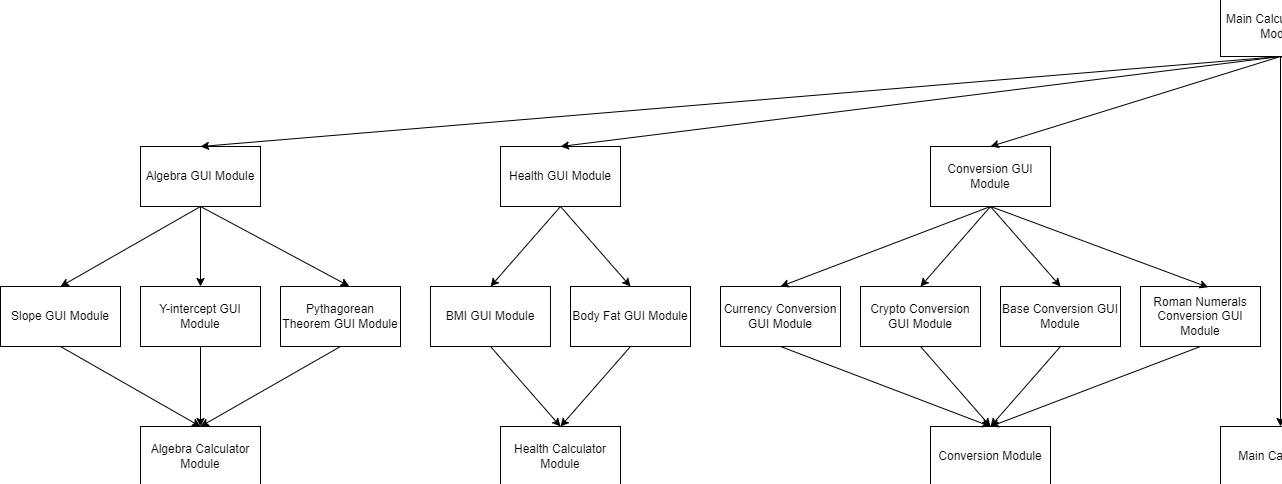
\includegraphics[scale=0.7, angle=270]{UsesHierarchy1.png}
%\caption{Use hierarchy among modules}
\label{FigUH}
\end{figure}

\begin{figure}[H]
\centering
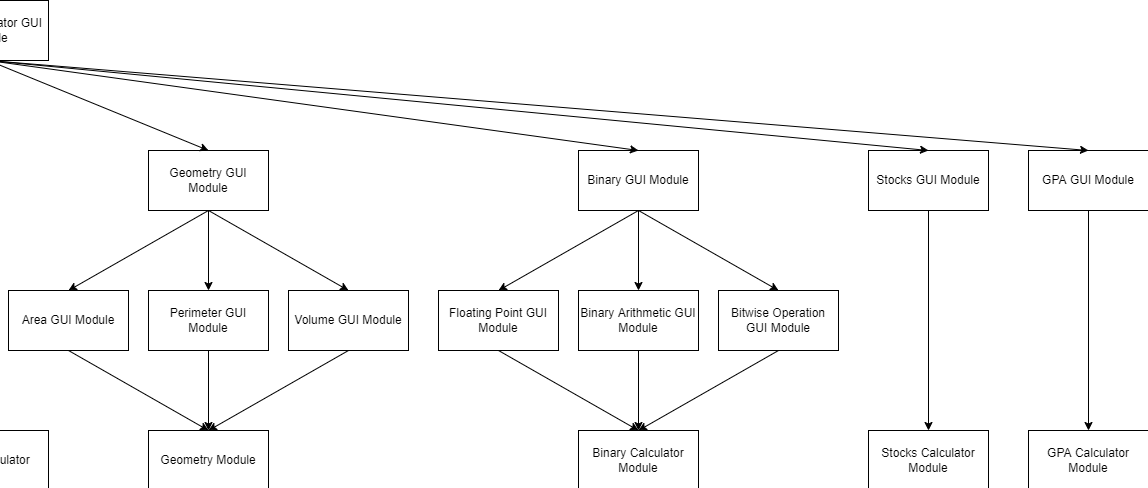
\includegraphics[scale=0.7, angle=270]{UsesHierarchy2.png}
\caption{Use hierarchy among modules}
\label{FigUH}
\end{figure}

%\section*{References}

\bibliographystyle {plainnat}
\bibliography {MG}

\end{document}
